\chapter{Anatomy of an AI coding agent}

\section{Engineering principles}

An inference request yields text or a proposed tool action. A harness translates a valid proposal into execution only after checking policy, then returns bounded observations to the model. The model does not inherit the authority of the operating system by itself. Working context holds the immediate goal, history and selected repository evidence; durable state lives outside the inference window. Planning may be explicit or implicit, and tool results can lead to revision, another call, escalation or termination.\src{O6,A9}

\section{Implementation approach}

Record task ID, baseline SHA, approved scope, attempt count and evidence paths before invocation. Read a failing test, inspect a symbol, propose a patch, run the test, and compare the resulting diff. Persist a concise checkpoint after each verified milestone. Distinguish tool failure from assertion failure and model refusal. Bound wall time and retry count independently of model behavior.

\section{Verification and limitations}

Success requires test evidence and an authorized diff; a timeout, policy denial, missing evidence or exhausted budget produces a non-success state. Do not treat an agent response as proof that an action occurred.

Figure~\ref{fig:d1} illustrates the conceptual flow from Engineering task to Authorized tools. The edges describe the proposed integration or control relationship, not undocumented internal calls.

\begin{figure}[htbp]\centering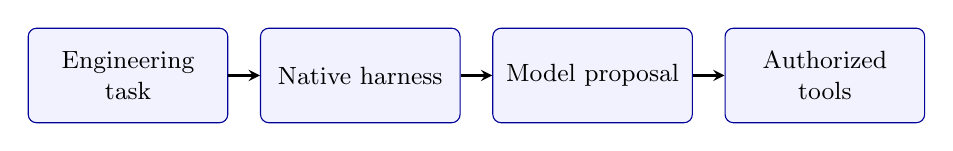
\begin{tikzpicture}[nodebox/.style={draw=blue!60!black,fill=blue!5,rounded corners=3pt,minimum height=12mm,text width=23mm,align=center,font=\small},>=stealth]
\node[nodebox] (n0) at (0.00,0.00) {Engineering task};
\node[nodebox] (n1) at (2.95,0.00) {Native harness};
\node[nodebox] (n2) at (5.90,0.00) {Model proposal};
\node[nodebox] (n3) at (8.85,0.00) {Authorized tools};
\draw[->,thick] (n0.east) -- (n1.west);
\draw[->,thick] (n1.east) -- (n2.west);
\draw[->,thick] (n2.east) -- (n3.west);
\end{tikzpicture}
\caption{Model, agent, framework and harness (conceptual view).}\label{fig:d1}\end{figure}

Figure~\ref{fig:d5} illustrates the conceptual flow from Intake to Observe / verify. The edges describe the proposed integration or control relationship, not undocumented internal calls.

\begin{figure}[htbp]\centering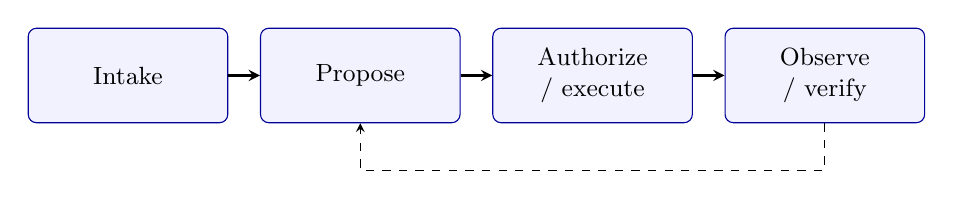
\begin{tikzpicture}[nodebox/.style={draw=blue!60!black,fill=blue!5,rounded corners=3pt,minimum height=12mm,text width=23mm,align=center,font=\small},>=stealth]
\node[nodebox] (n0) at (0.00,0.00) {Intake};
\node[nodebox] (n1) at (2.95,0.00) {Propose};
\node[nodebox] (n2) at (5.90,0.00) {Authorize / execute};
\node[nodebox] (n3) at (8.85,0.00) {Observe / verify};
\draw[->,thick] (n0.east) -- (n1.west);
\draw[->,thick] (n1.east) -- (n2.west);
\draw[->,thick] (n2.east) -- (n3.west);
\draw[->,dashed] (n3.south) -- ++(0,-.6) -| (n1.south);
\end{tikzpicture}
\caption{Agent execution lifecycle (conceptual view).}\label{fig:d5}\end{figure}

\section{Chapter conclusion}

Apply the stated verification criteria before expanding the scope of this workflow. Record deviations, evidence and unresolved risks in the task record.
